\section{Diagramas de Sequ�ncia \label{diagramas_sequencia}}

\subsection{Carregamento do v�deo \label{seq_carrega}}

\begin{figure}[h|top]
 \centering
 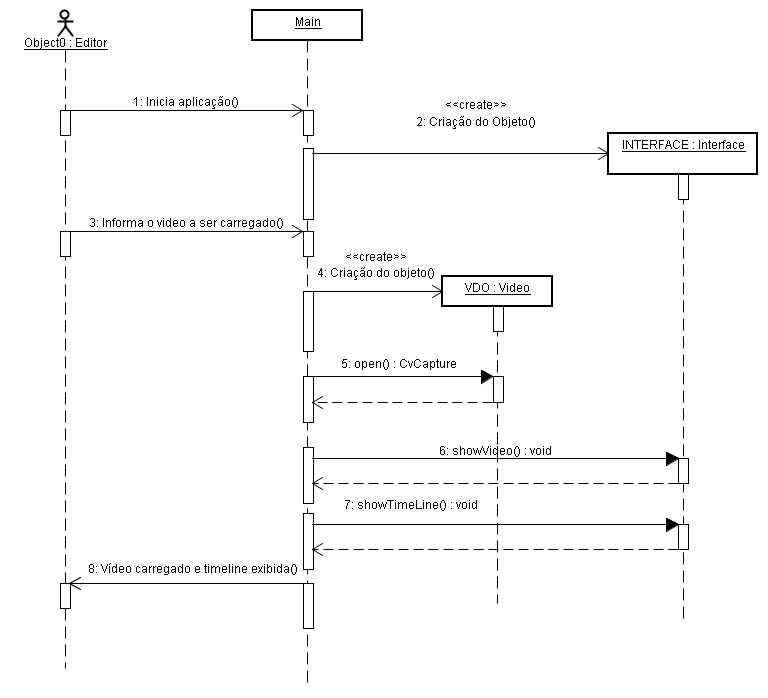
\includegraphics[width=1.0\linewidth]{imagens/seq_main.PNG}
 \caption{Diagrama de sequ�ncia para carregamento do v�deo.}
 \label{img_seq_main}
\end{figure}

\subsection{Detec��o de transi��es geral \label{seq_detecta_geral}}

\begin{figure}[h|top]
 \centering
 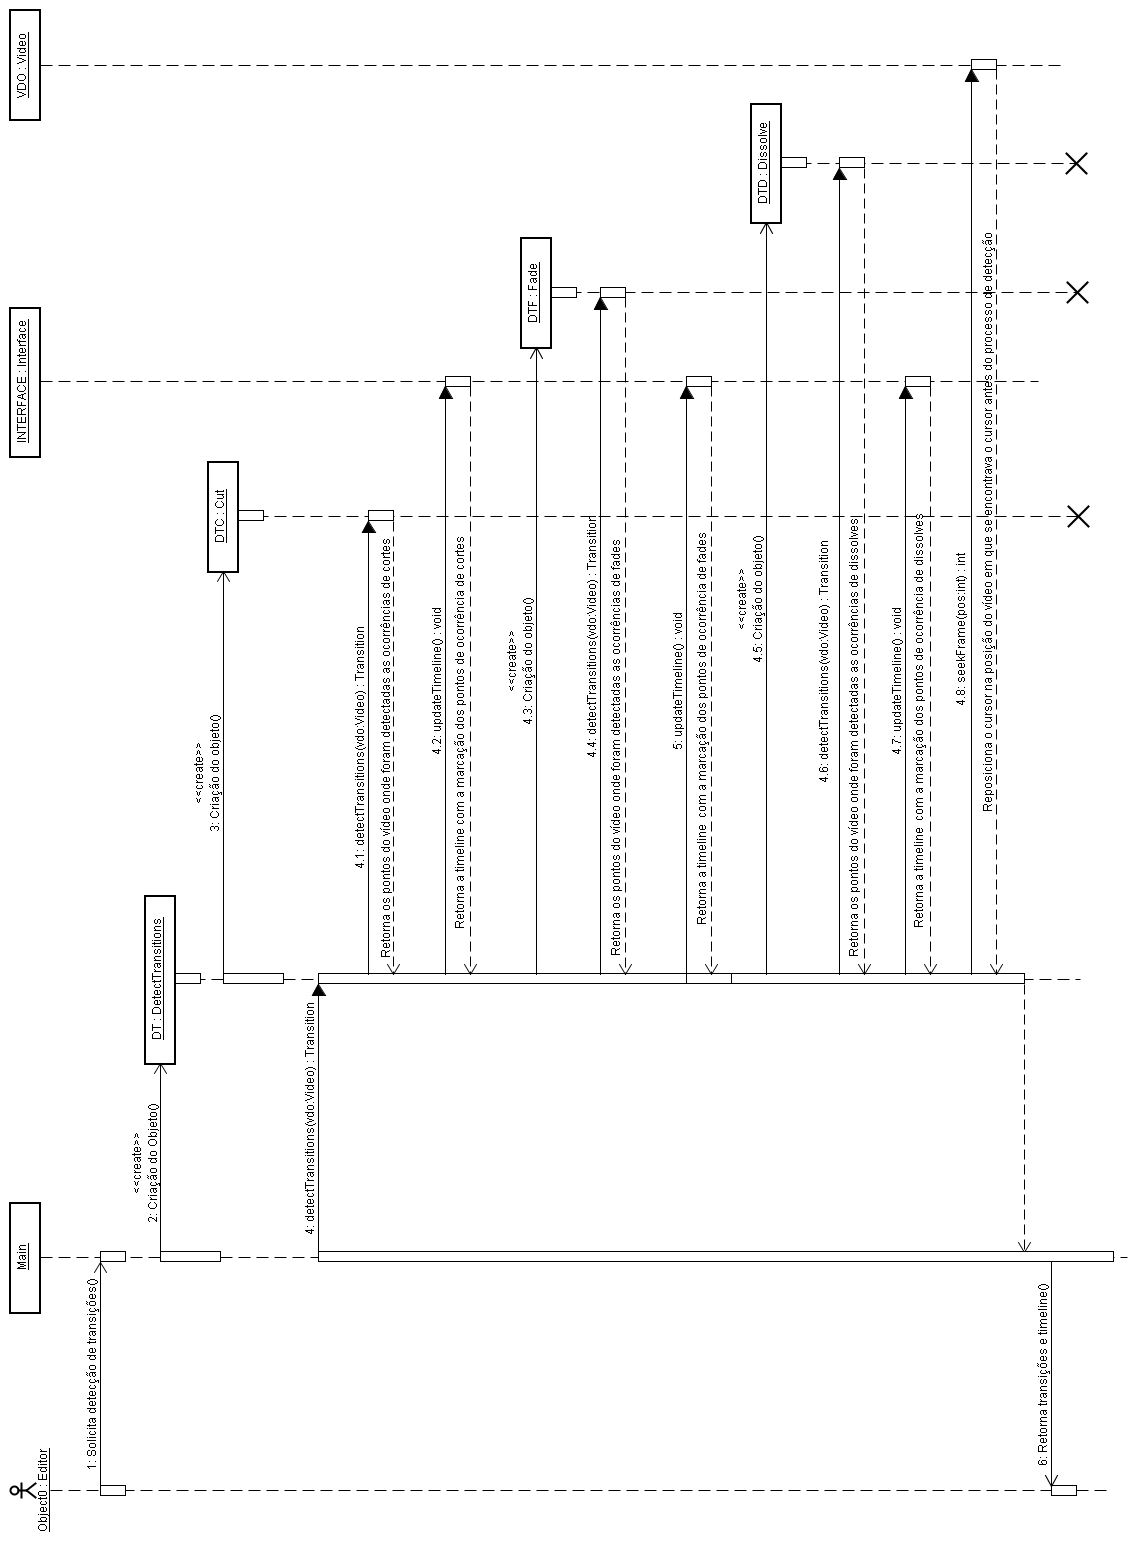
\includegraphics[width=1.0\linewidth]{imagens/seq_detecta.PNG}
 \caption{Diagrama de sequ�ncia para detec��o de transi��es.}
 \label{img_diagrama_de_classes}
\end{figure}

\subsection{Detec��o de Cortes \label{seq_cortes}}

\begin{figure}[h|top]
 \centering
 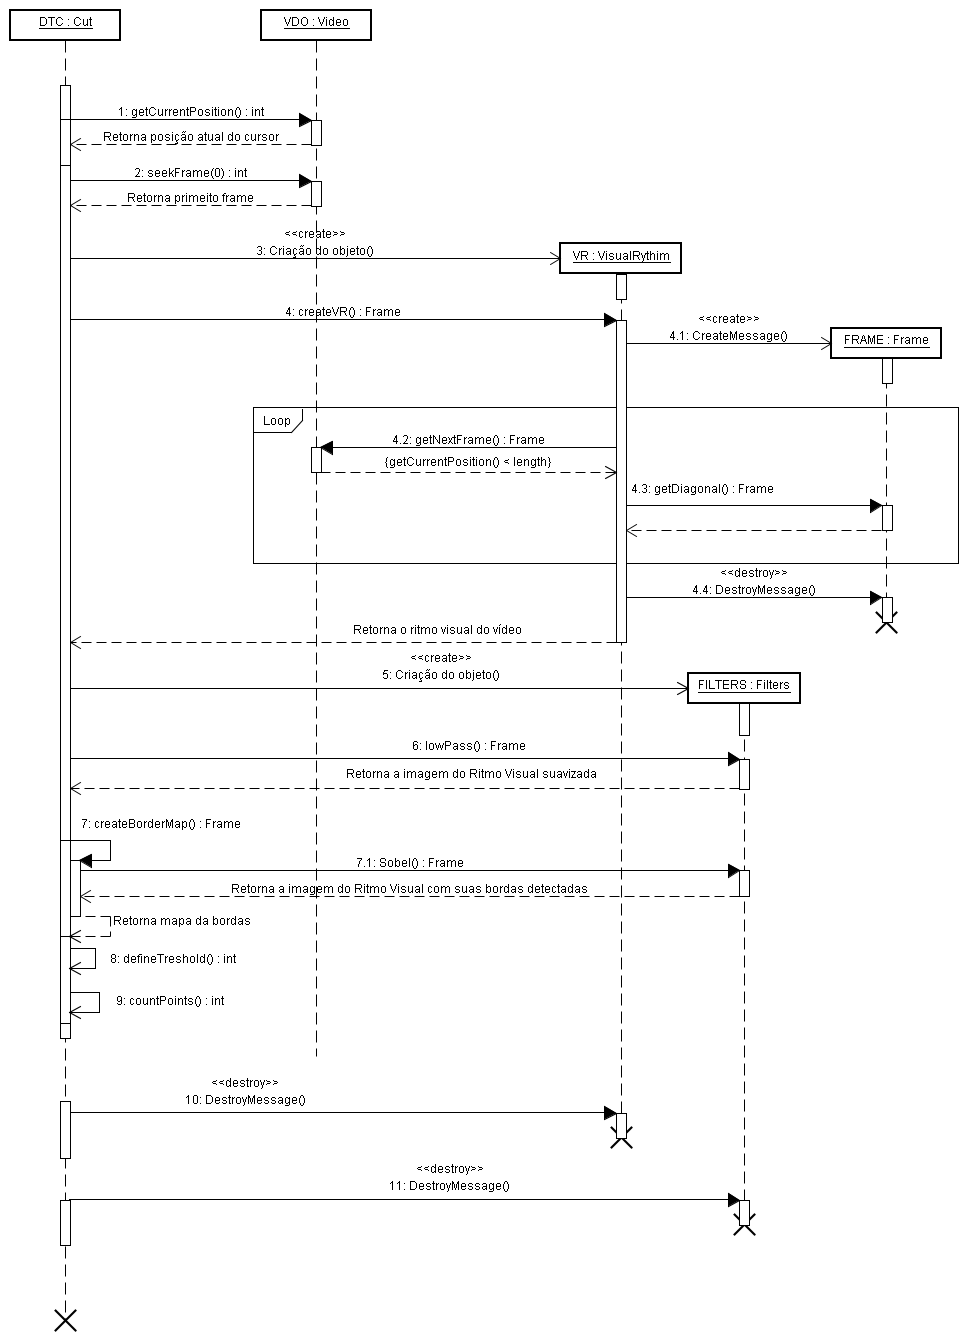
\includegraphics[width=1.0\linewidth]{imagens/seq_cortes.PNG}
 \caption{Diagrama de sequ�ncia para detec��o de cortes.}
 \label{img_diagrama_de_classes}
\end{figure}

\subsection{Detec��o de Fades \label{seq_fades}}

\begin{figure}[h|top]
 \centering
 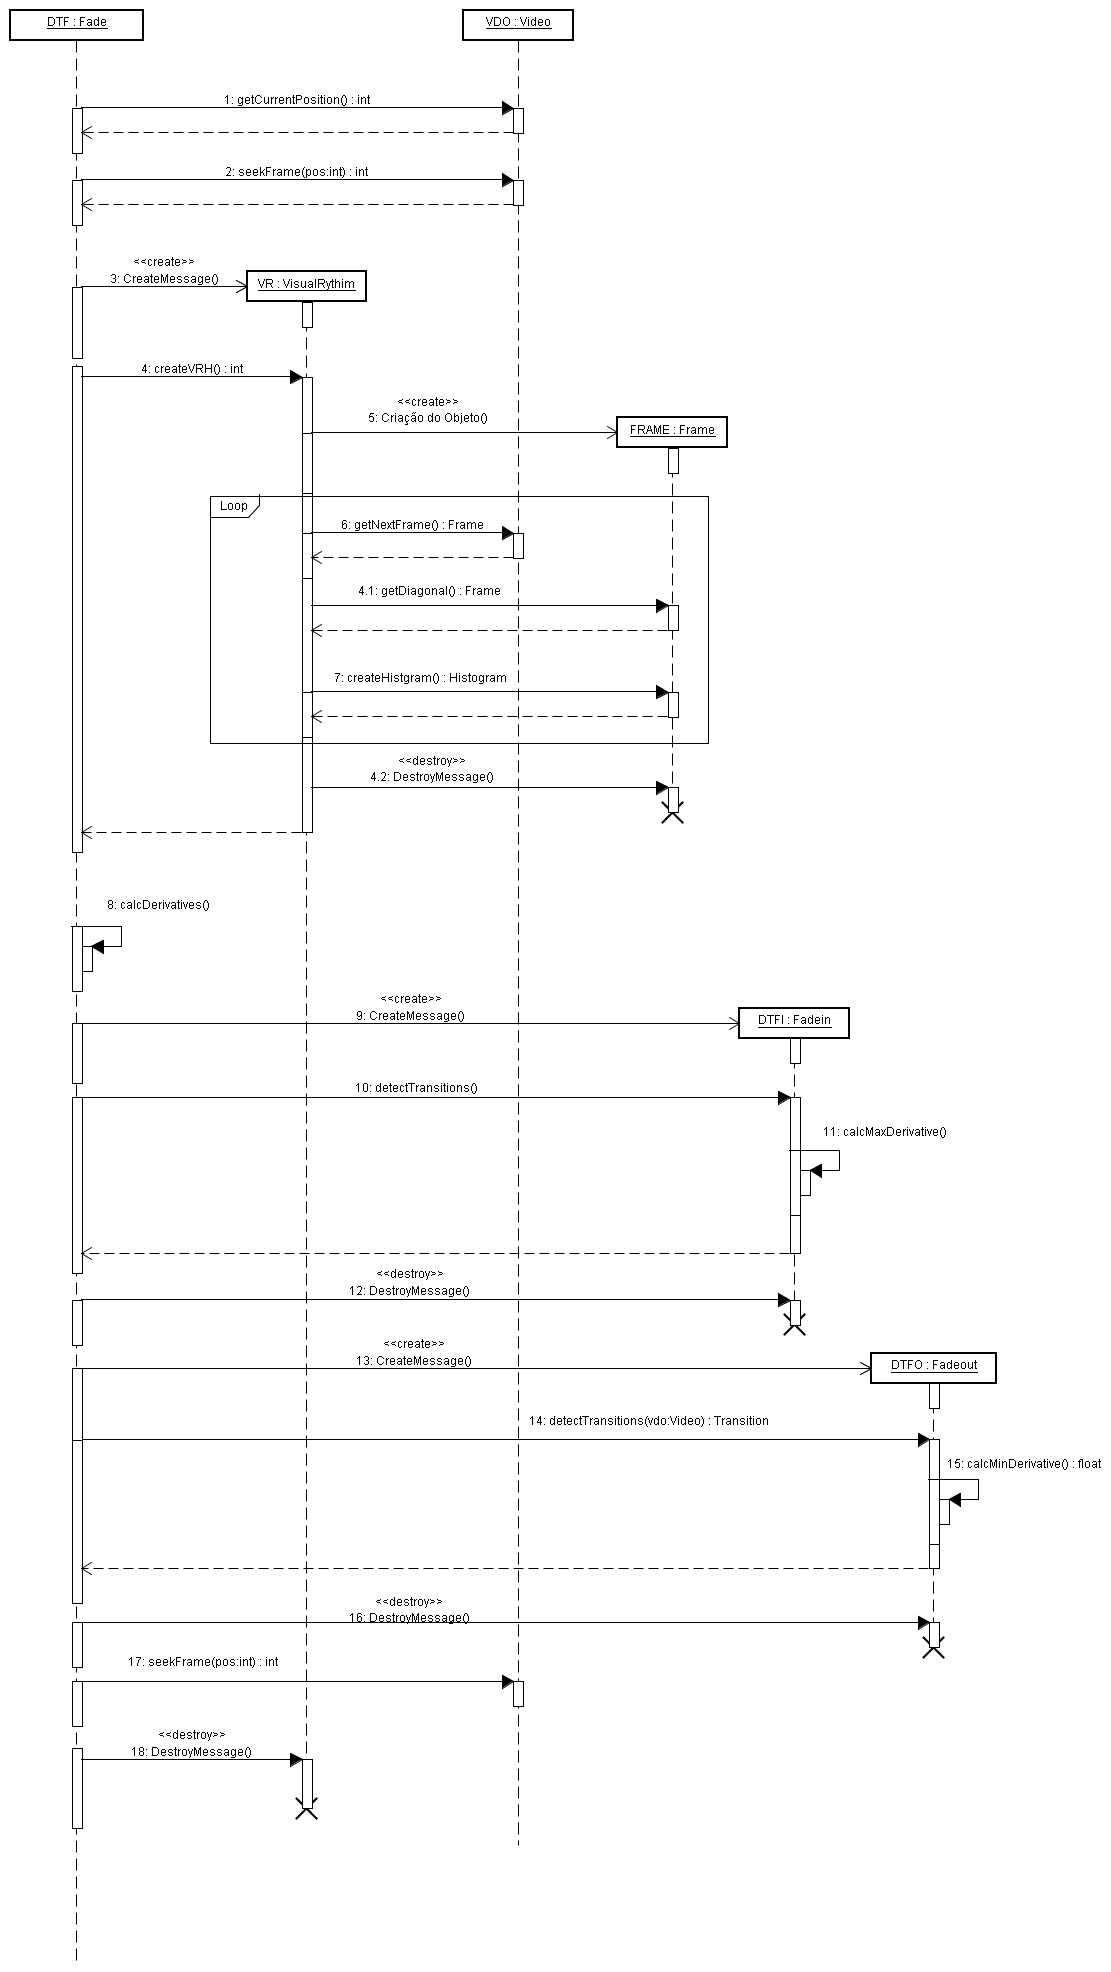
\includegraphics[width=1.0\linewidth]{imagens/seq_fade.PNG}
 \caption{Diagrama de sequ�ncia para detec��o de fades (fade-in e fade-out).}
 \label{img_diagrama_de_classes}
\end{figure}

\subsection{Detec��o de Dissolves \label{seq_dissolves}}

\begin{figure}[h|top]
 \centering
 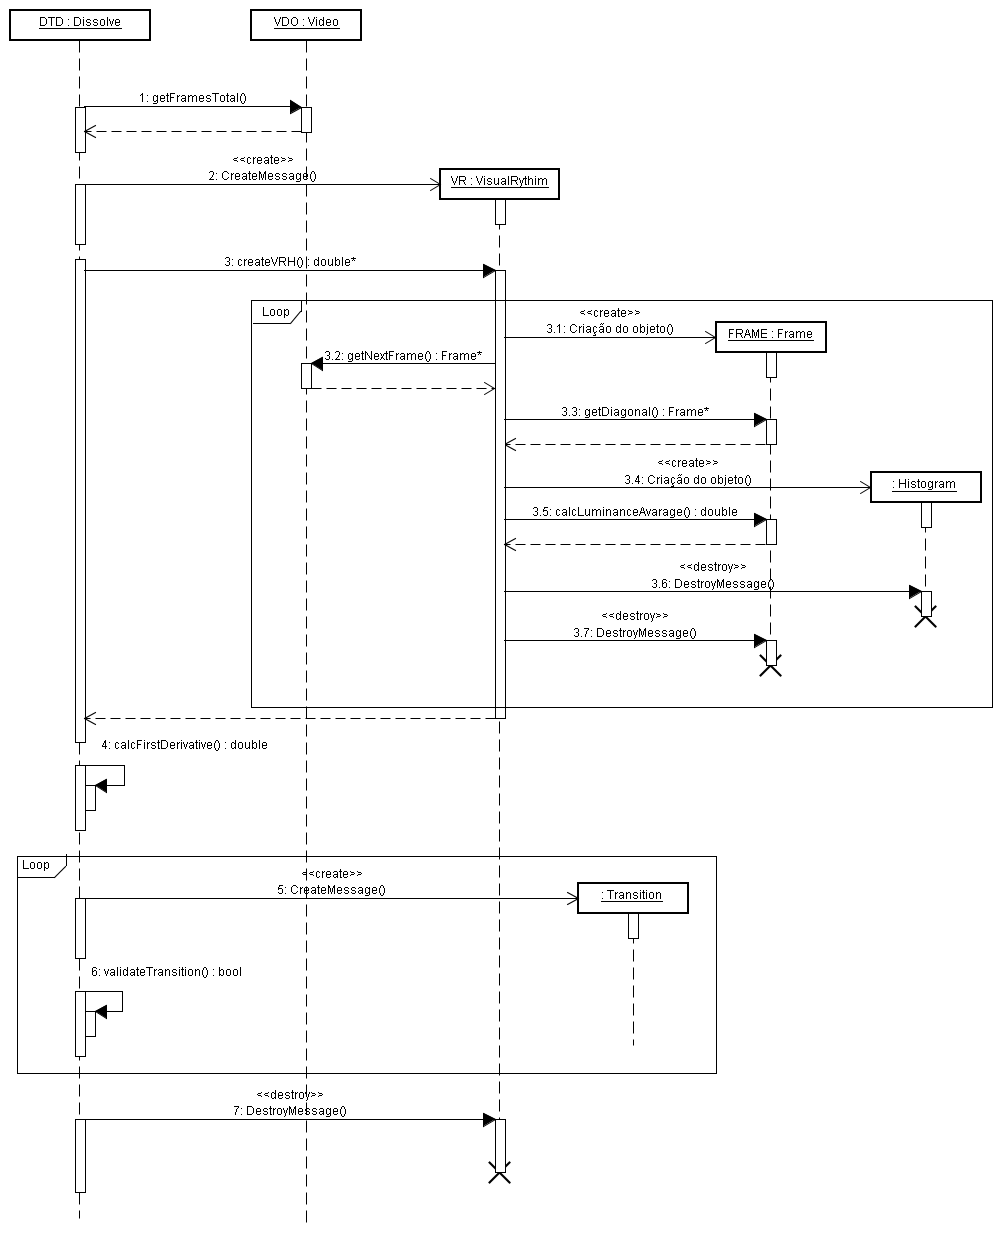
\includegraphics[width=1.0\linewidth]{imagens/seq_dissolve.PNG}
 \caption{Diagrama de sequ�ncia para detec��o de dissolves.}
 \label{img_diagrama_de_classes}
\end{figure}

\subsection{Edi��o de v�deo \label{seq_edicao}}

\begin{figure}[h|top]
 \centering
 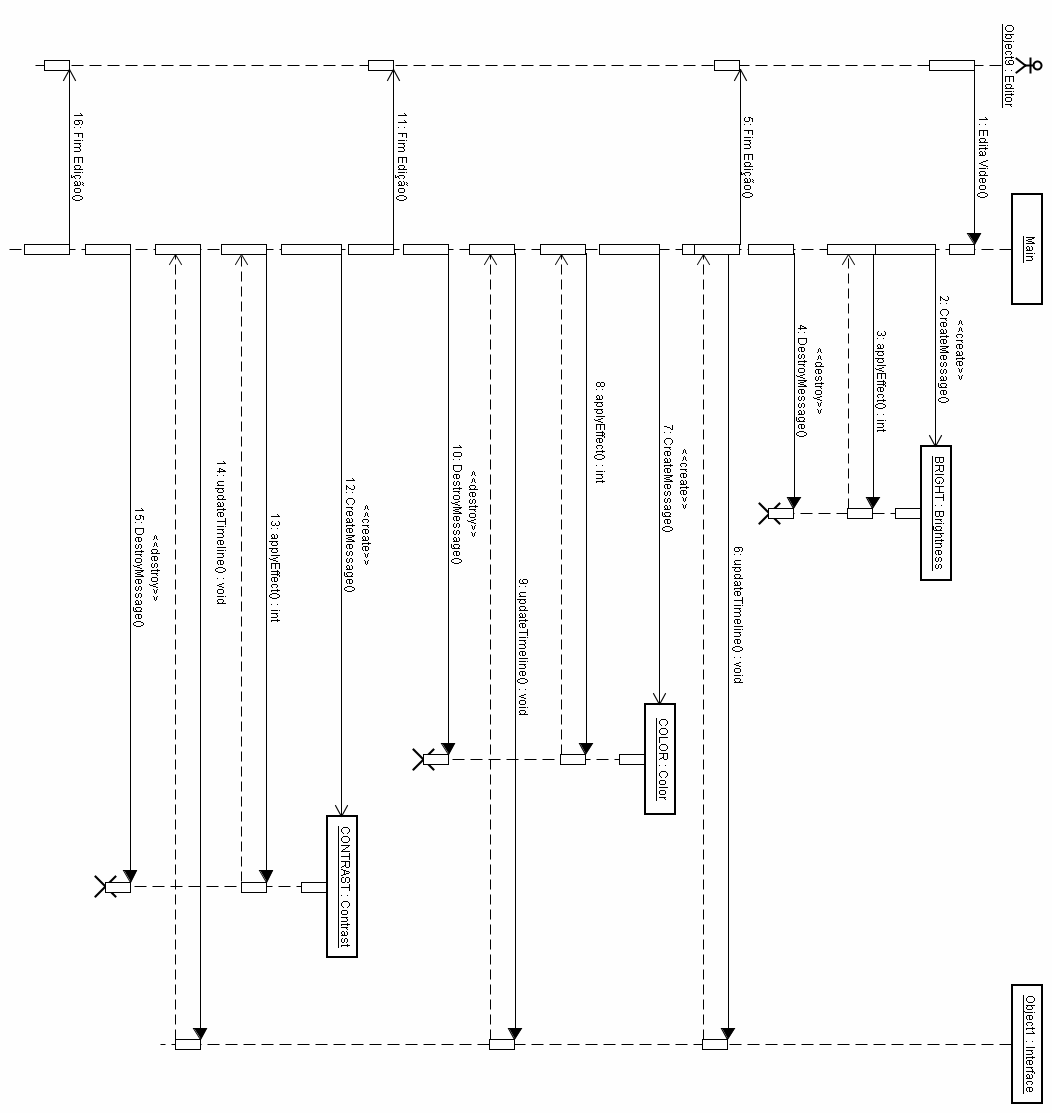
\includegraphics[width=1.0\linewidth]{imagens/seq_edicao.PNG}
 \caption{Diagrama de sequ�ncia para edi��o de v�deo.}
 \label{img_diagrama_de_classes}
\end{figure}
